\section{Classifier Design}
\label{sec:ClasDes}
As stated in the introduction, a classifier had to be build for two different cases. For both cases, a similar design approach was used. \begin{enumerate}
	\item Investigate amount of data and use the theory to choose an initial representation method
	\item Train simple classifiers based on the chosen representation method
	\item Perform evaluation
	\item If the performance does not meet the requirements, go back to the theory
	\item If the performance meets the requirements, optimise the system
\end{enumerate}
This approach is visualised in figure \ref{fig:case_design}.
\begin{figure}[H]
	\centering
	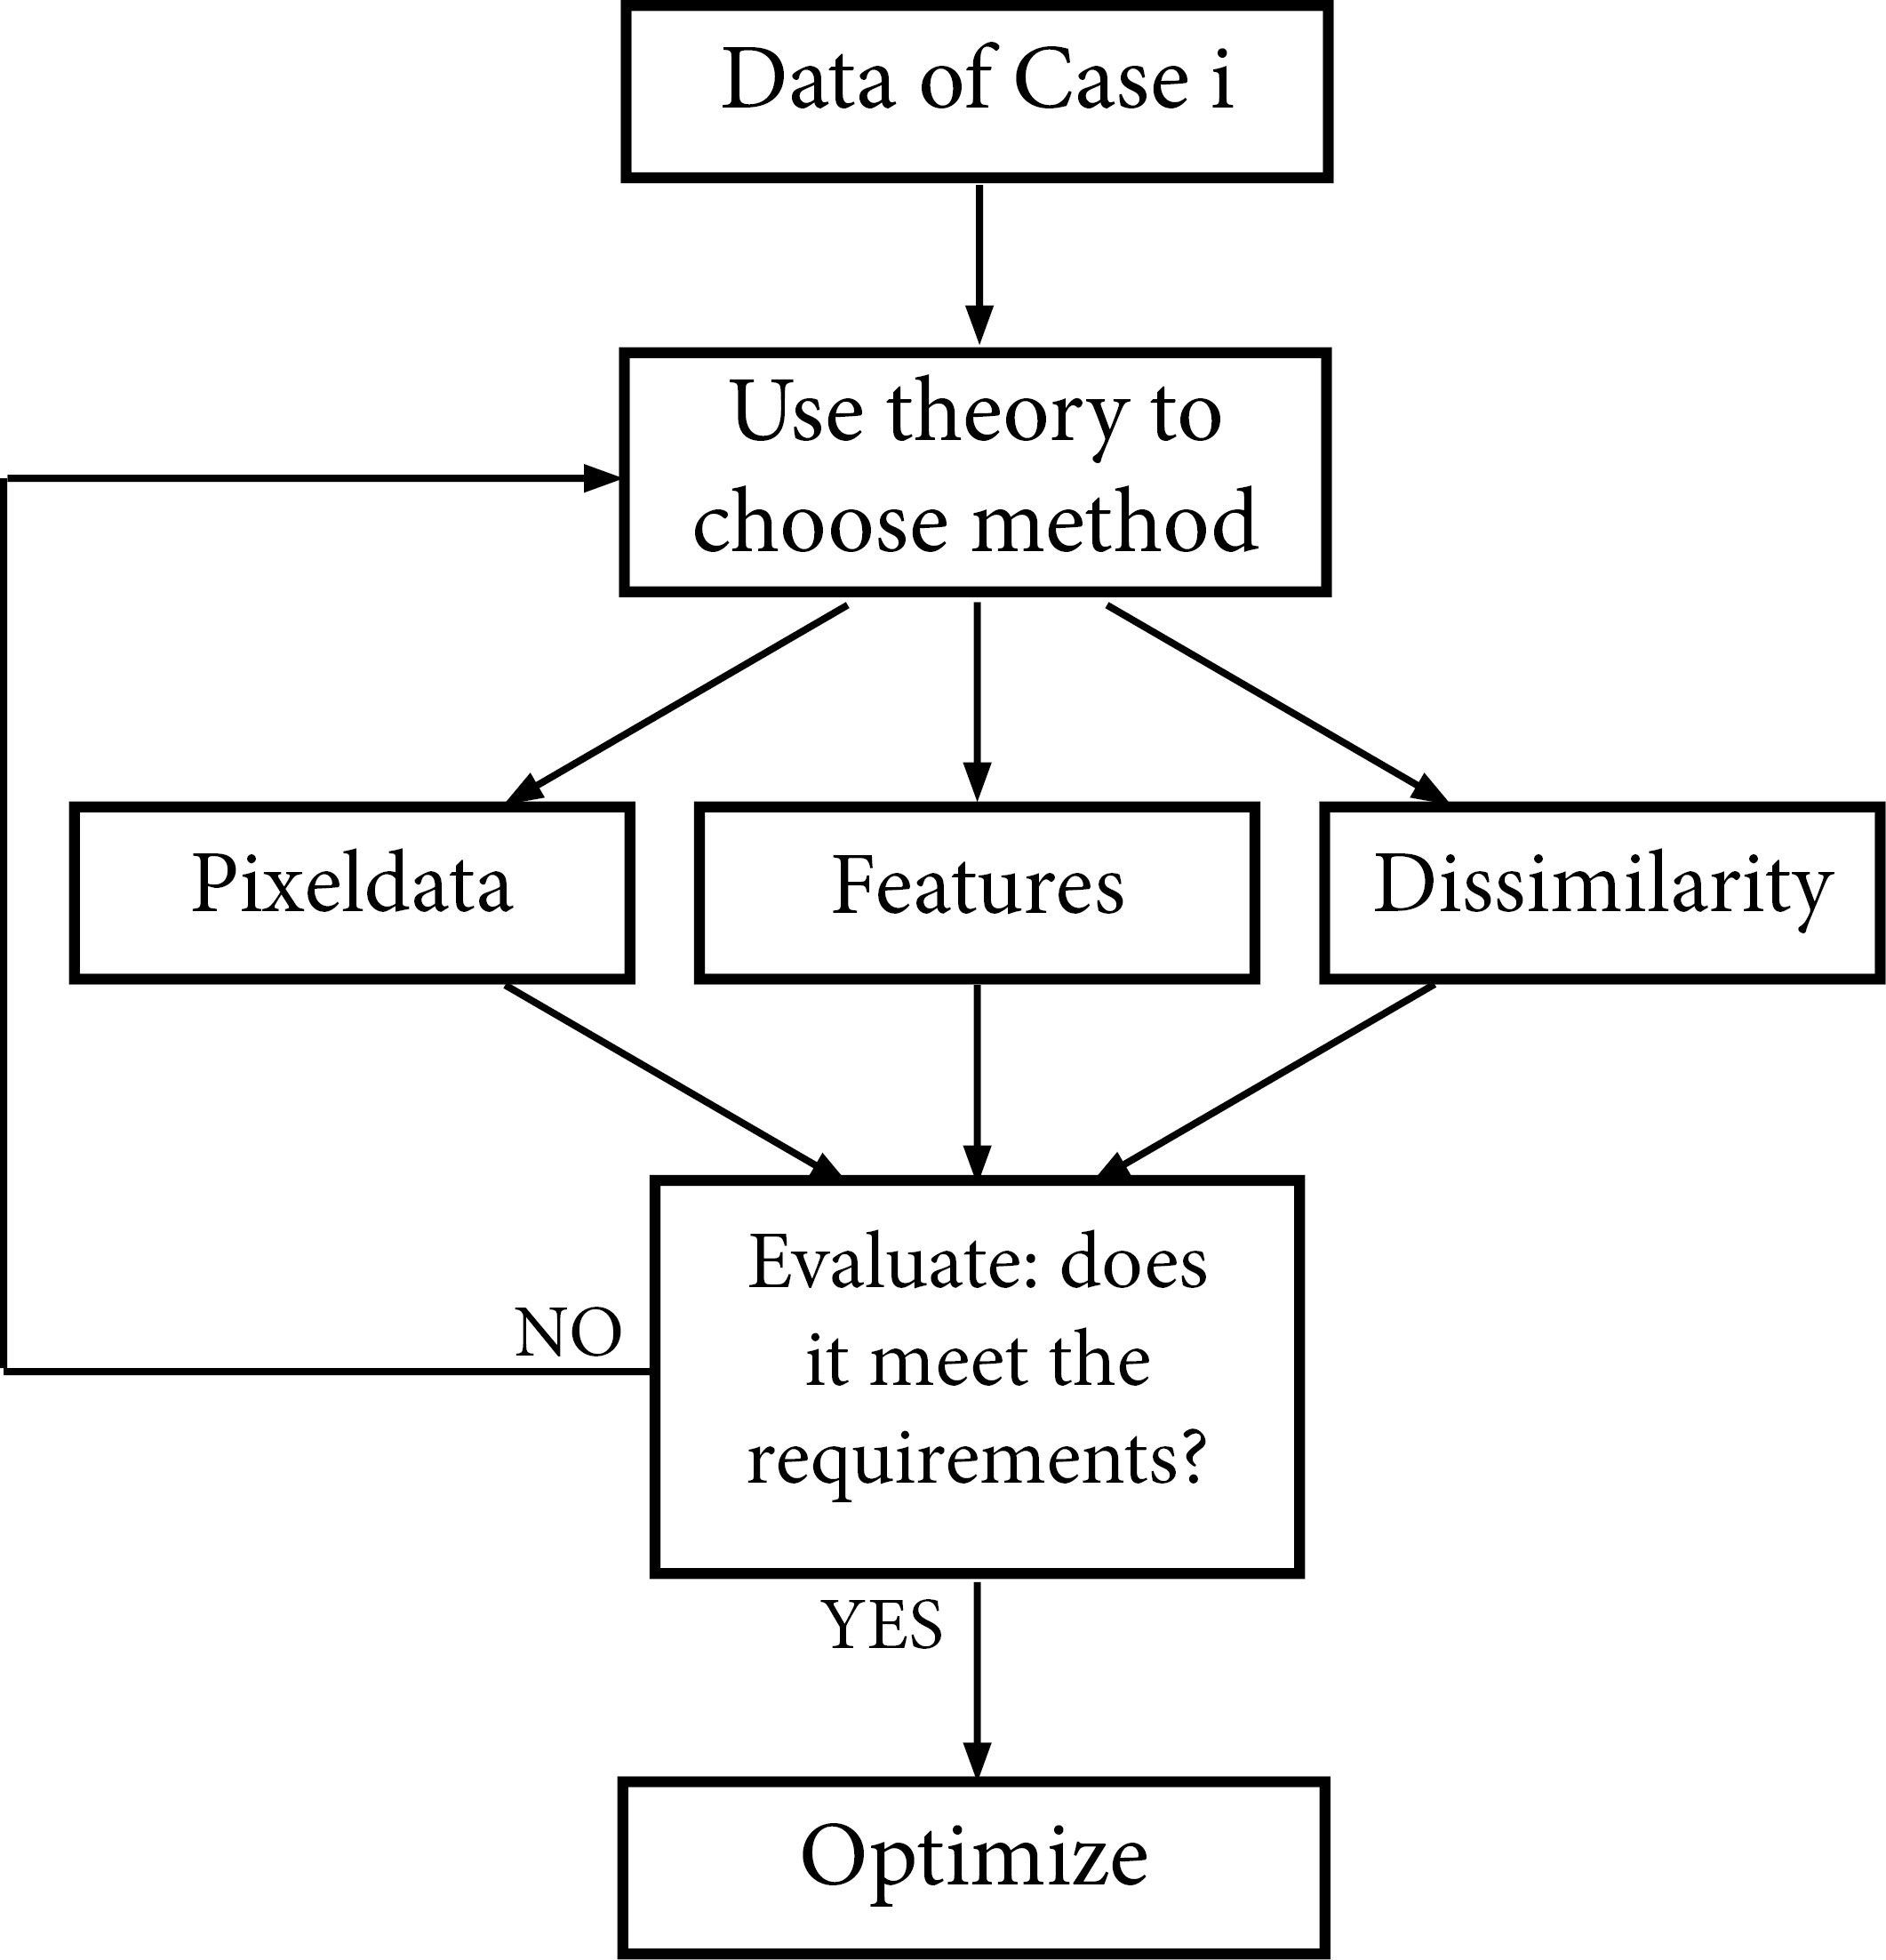
\includegraphics[scale=0.55]{images/Case_Design.jpg}
	\caption{Design-process to determine the best representation method for each of the two cases described in the Introduction.}
	\label{fig:case_design}
\end{figure}
\noindent The image processing described in chapter \ref{sec:ImPros} was kept the same for both cases, since it is a very subtle processing and will benefit all potential methods.

\subsection{Case 1}
\label{sec:Case1}
\textbf{Case Summary:} Design a system for training on all cheques at once. The system must be able to correctly classify the handwritten digits after being trained on at least 200 objects per class.\\
\\
\noindent This case has a lot of data available. A wise choice to start would be to use a pixeldata representation, potentially in combination with some form of feature reduction. \\
Smag

\subsection{Case 2}
\label{sec:Case2}
\textbf{Case Summary:} Design a system for training on each batch of cheques to be processed. The system must be able to correctly classify the handwritten digits after being trained on a maximum of 10 objects per class.\\
\\
\noindent The amount of data available in this case poses some restrictions. While a pixel-data representation worked very well in Case 1, it is likely to have too little data to work with in this case. Some more prior knowledge is needed to handle these batches of cheques. One way of doing this is by letting the system recognize certain distinct properties of the digits. A straight-forward way of doing this is by using a feature representation of the objects. A more abstract way is using a dissimilarity representation.
\\
\subsubsection*{Representation by Features}
To start out, features were chosen as the best representation for this case. The function \texttt{im\_features} from the prtools-toolbox was used to compute 14 different features of all the images in the pre-processed database. Because the amount of features is relatively high compared to the amount of data that is used, some form of feature reduction needs to by applied. MatLab's forward feature selection (\texttt{featself}) was used initially to get a sense for the features that should be used and the features that could be omitted. This was done for four cases; with and without scaling of the data, and with and without implementing a separate test-set in the \texttt{featself} function. The resulting performance can be seen in figure \ref{fig:featsel_perf}
\begin{figure}[H]
	\centering
	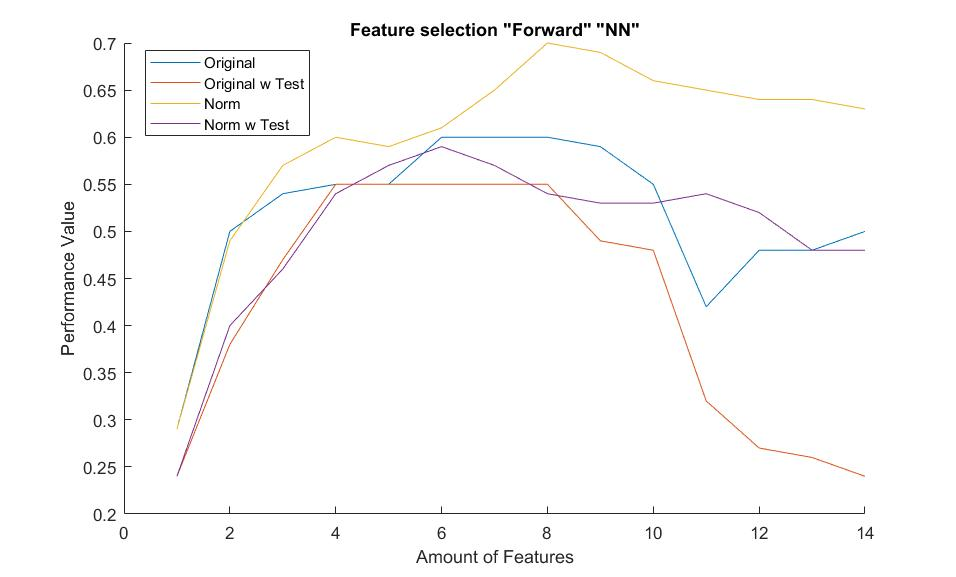
\includegraphics[scale=0.45]{images/featsel_perf.jpg}
	\caption{Performance of features selected by forward feature selection. Both scaling and non-scaling, and with or without test-set are shown.}
	\label{fig:featsel_perf}
\end{figure}
\noindent As can be seen in the figure, there are a lot of differences between the different parameters. There appears to be an optimal amount of features however, somewhere between 4 and 12. In order to get a better grip on which features to use, different feature selection strategies were compared. \todo{Ik heb hier nog bij gezet dat ik ook andere dingen dan forward heb getest.} After the forward selection, the backward and the plus-2-takeaway-1 were tested. This is was done for both the '1-Nearest Neighbor' and the 'Summed Mahalanobis distances' criterion. All these methods indicated that there was an optimum somewhere between 4 and 12 features. However there seemed to be no correlation between which of the features belonged to this optimal set. Therefore a brute force approach was taken. Each possible combination between 3 and 14 features was used for an error-calculation (using the \texttt{testc}  function of PRTools) of four different classifiers (Fischer's Classifier, Linear Classifier, Nearest Mean Classifier and a Nearest Mean Classifier trained on normalized data). After running this setup overnight, the following results were obtained: (see figure \ref{fig:feat_bf_error}).
\begin{figure}[H]
	\centering
	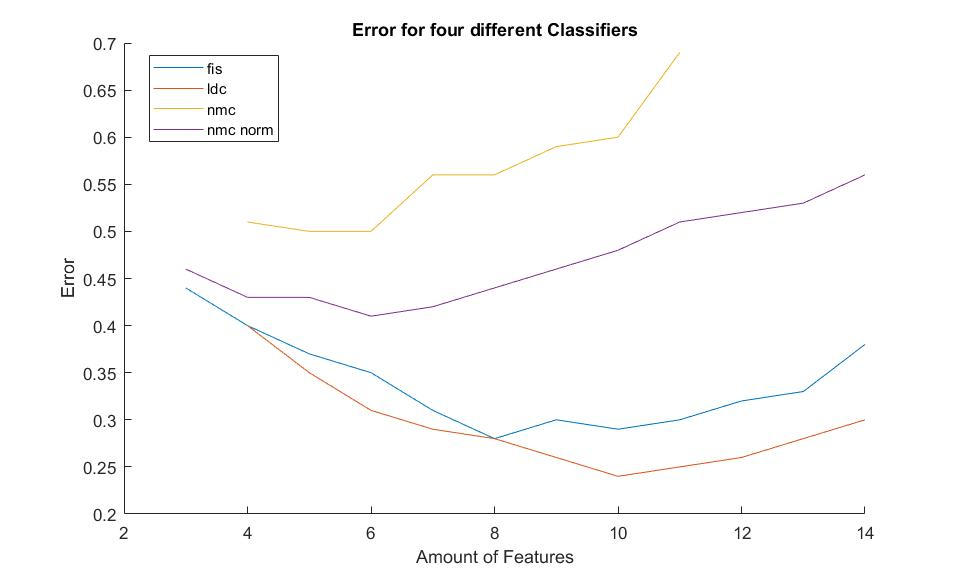
\includegraphics[scale=0.45]{images/feat_bf_error.jpg}
	\caption{Error of different combinations of features for four different trained classifiers; Fischer's (\texttt{fischerc}), Linear Bayes-Normal (\texttt{ldc}), Nearest Mean (\texttt{nmc}) and a normalised version of Nearest Mean.}
	\label{fig:feat_bf_error}
\end{figure}
\noindent This figure shows the lowest error obtained with a certain amount of features. It suggests the optimal amount is 10. It also shows that the Linear Classifier will probably perform best, although even its best error is not under the 25 percent yet. \\
\todo{Vanaf hier heb ik de tekst een beetje veranderd}Next, for the LDC classifier only, these 10 features were tested on different datasets. The result of this was a big fluctuation in errors between datasets, which implies that the set of 10 features were only optimal for one particular dataset. Therefore another brute force approach was used to test all possible combinations of 9 to 12 features on different datasets. In figure \ref{fig:feat_jumps} the error of every combination of 9 features can be seen. Very noticeable are the large drops and jumps in the graph, visualised with the orange line below it. After close inspection of the used features at these points, it was discovered that every increase in error corresponded to the same four features being added, namely 'Convex Area', 'Convex Hull', 'Convex Image' and 'Eccentricity'. A similar pattern was recognized in the other results. It was decided to omit these features, leaving the final dataset with the desired amount of 10 features.
\begin{figure}[H]
	\centering
	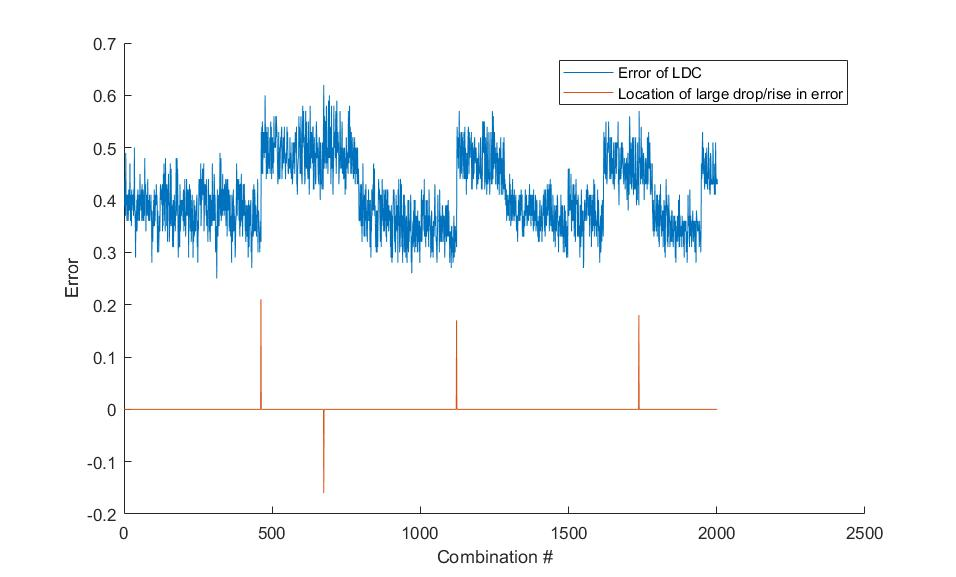
\includegraphics[scale=0.45]{images/feat_jumps.jpg}
	\caption{Error of the LDC-classifier for each possible combination of 10 out of 14 features. The orange line indicates places with a large increase or decrease in error-value.}
	\label{fig:feat_jumps}
\end{figure}
\noindent At this time, the complete system consisted of a Linear Classifier (LDC) trained on the dataset from which 10 features were selected. Sadly though, testruns of the algorithm yielded an error of 30\%. Since this was too low to meet the requirements, a different approach was taken. \\
\subsubsection*{Representation by Dissimilarity}
It was decided that more information needed to be intrinsic in the system in order for it to be able to correctly classify the digits with the small trainingset Case 2 provides. Going back to the theory, dissimilarity-representation seemed to be able to do this. By picking a few representative examples of each digit by hand (the prototypes) and calculating the distance of the remaining objects to these prototypes, correct classification should be possible. \\
\noindent To get a first test of this principle, it was tried to first filter out all some digits. 90 samples per class were taken, two representative ones were chosen, and the distance between all objects and these three zeros was calculated using MatLab's \texttt{proxm} function. 
\begin{figure}[H]
	\centering
	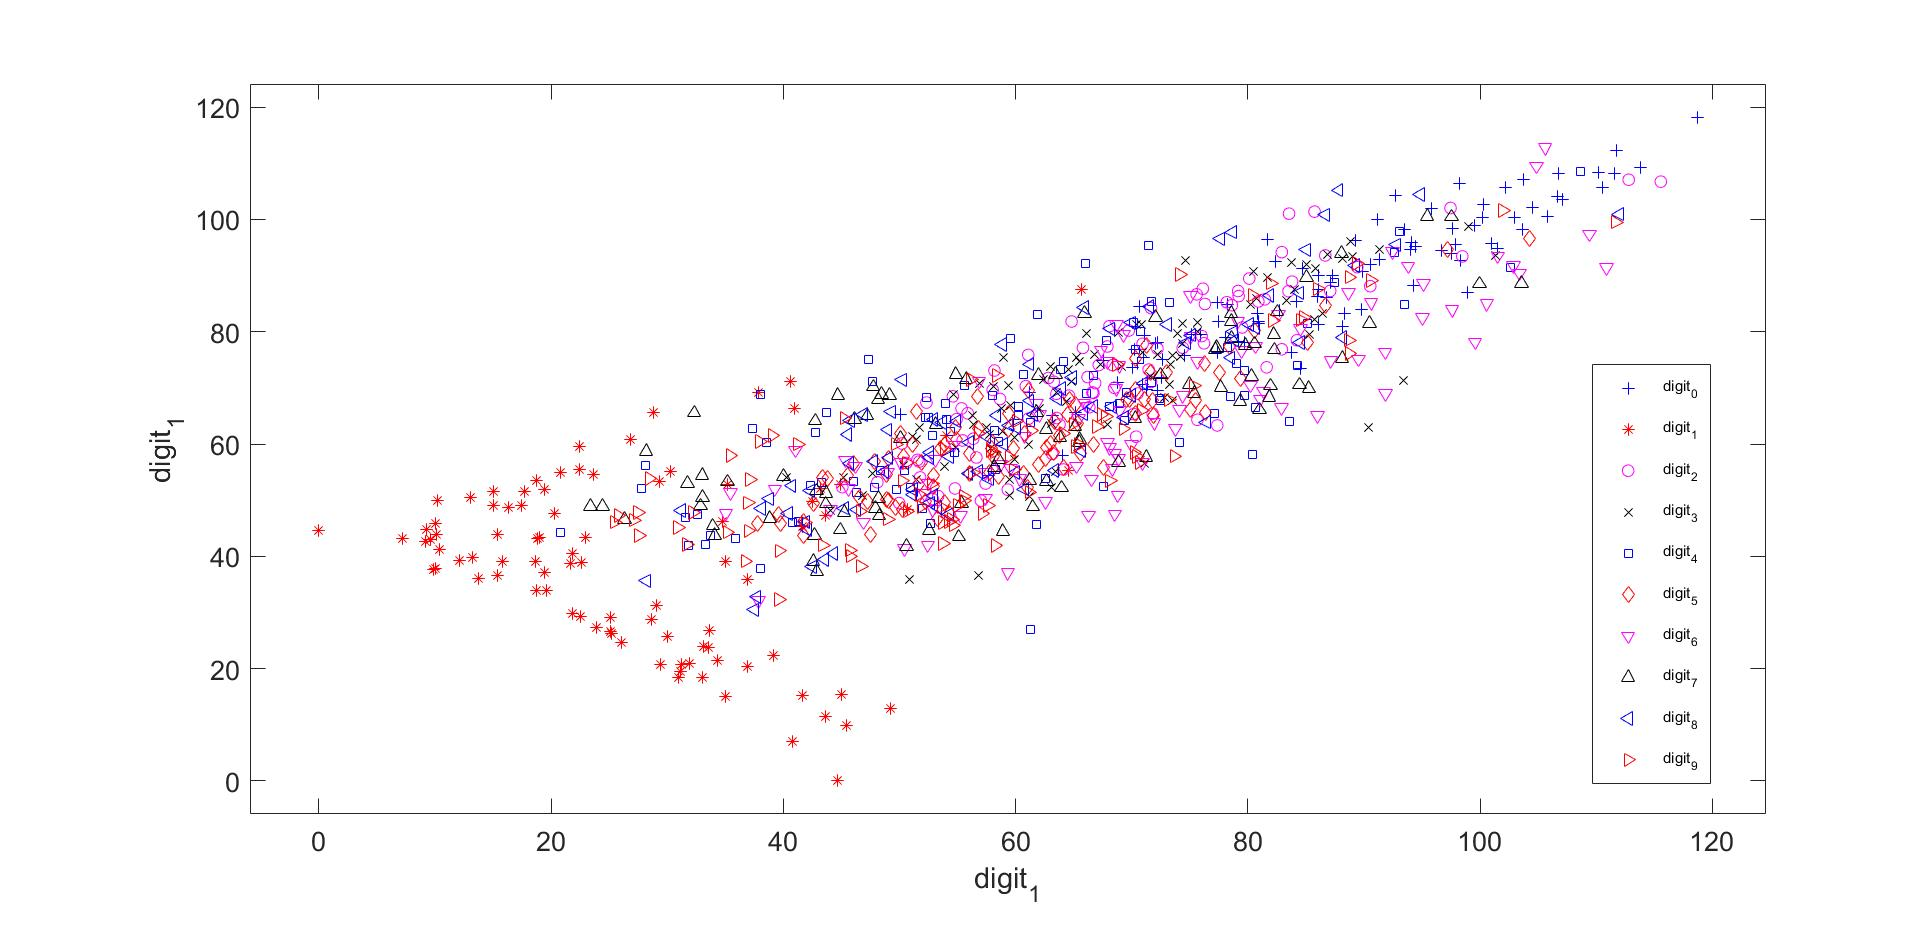
\includegraphics[width = 0.9\textwidth]{images/dissim_two_ones.jpg}
	\caption{Dissimilarity of 90 samples per class to two digit-one prototypes, using city-block distances.}
	\label{fig:dissim_two_ones}
\end{figure}
In figure \ref{fig:dissim_two_ones} a clear grouping of all the ones can be observed, and this group can be separated from the rest of the objects easily. This was done for various distance measures. As can be seen in figure \ref{fig:dissim_bar_dist} a few distance measures perform comparable, but city-block seemed to be the most consistent over different training sets. \todo{VERWIJZEN NAAR PAPER, en zeggen dat het in image goed werkt} \\
\begin{figure}[H]
	\centering
	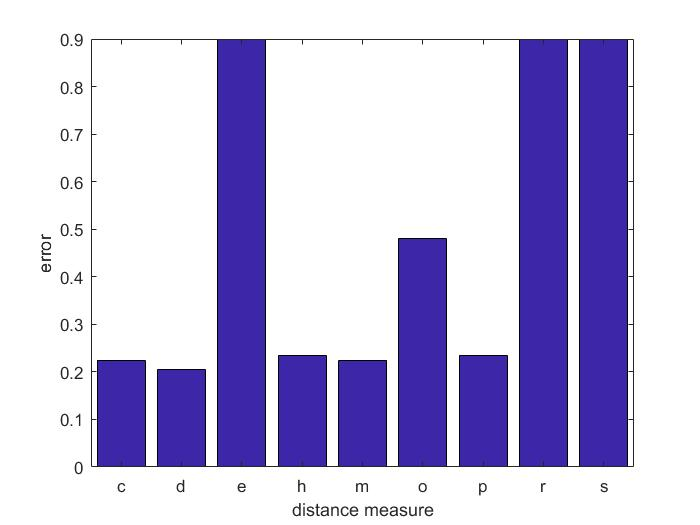
\includegraphics[width = 0.9\textwidth]{images/dissim_bar_dist.jpg}
	\caption{Error of \texttt{ldc} classifier, using different distance measures.}
	\label{fig:dissim_bar_dist}
\end{figure}

\noindent The next step is to try this with every digit. Ten samples per class were taken, and in stead of selecting the prototypes manually, all objects were given as prototypes. This meant a dataset of 100 samples, each of them having 100 features. Now a decision must be made on what classifier to use. Because of the high dimensionality of the feature space and the relative low amount of samples, the more complex classifiers tend to 

fuck up.

\begin{figure}[H]
	\centering
	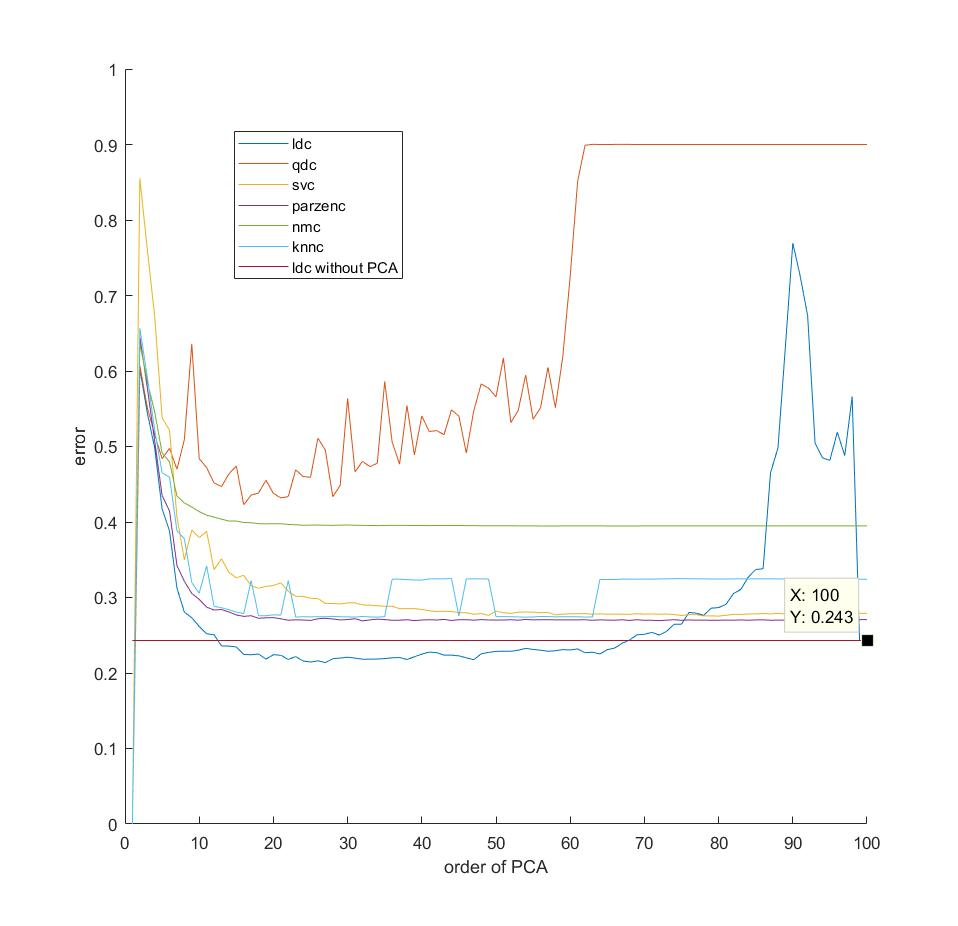
\includegraphics[width = 0.9\textwidth]{images/dissim_all_class.jpg}
	\caption{Error of different classifiers, using different orders of PCA.}
	\label{fig:dissim_all_class}
\end{figure}

\begin{figure}[H]
	\centering
	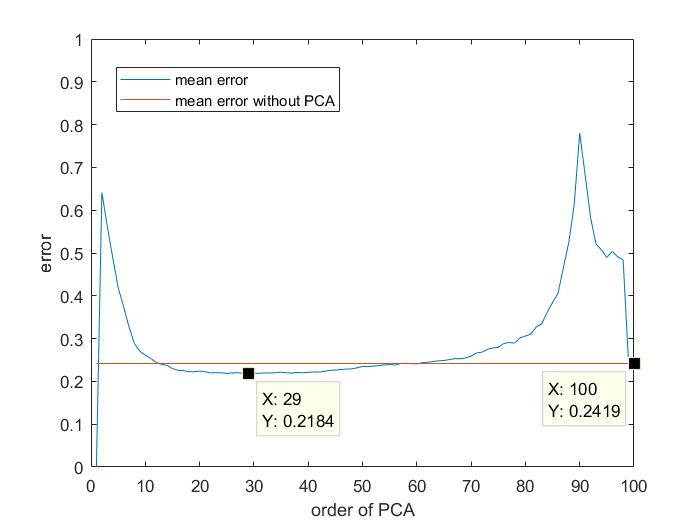
\includegraphics[width = 0.9\textwidth]{images/dissim_ldc_mean.jpg}
	\caption{Average error of ten test stets of \texttt{ldc}.}
	\label{fig:dissim_ldc_mean}
\end{figure}


